A system is judged by the quality of the services it offers and its ability to function reliably. Even though the reliability of operating systems has been studied for several decades, it remains a major concern today. The characteristics of operating systems which make them unstable are size and complexity. 
\\
Software reliability studies shows that 6 to 16 bugs/1000 lines can be found within a typical module~\cite{Basili:1984:SEC:69605.2085}. The Linux kernel has over 15 million lines of code. If we assume minimum estimate, Linux kernel may contain 90,000 bugs. Researchers have shown that device drivers has more bugs than the rest of the kernel~\cite{Chou:2001:ESO:502034.502042}. Considering the fact that the operating system predominantly consists of device drivers, the bugs in device drivers make the operating system unreliable~\cite{Chou:2001:ESO:502034.502042}.

\pagebreak

\section {Problem Statement}

The reliability of the system is influenced by the number of bugs in the device driver and the system should have small number of bugs in the device driver code. However, fixing all the bugs is difficult since bug fixes might introduce new lines of code resulting in new bugs. 
\\
Modern operating systems provide isolation from bugs using memory protection. Memory protection is a way to control memory access rights. It prevents a process from accessing memory that has not been allocated to it. Memory protection prevents a bug within a process from affecting other processes, or the operating system~\cite{Denning:1970:VM:356571.356573, Galvin}. Linux kernel modules do not have the same level of isolation the user level applications have. Unlike user applications, Linux kernel has hundreds of procedures linked together. As a result, any portion of the kernel can access and potentially overwrite any kernel data structure used by an unrelated component. Such a non-existent isolation between kernel and device driver causes a bug in device drivers to corrupt the memory of the other kernel components. This memory corruption might lead to system crash. The underlying cause of unreliability in the operating system is the lack of isolation between device driver and Linux kernel.
\\
In the past, solutions to increase the reliability of a system running monolithic kernel, based on virtualization has been proposed by LeVasseur et. al.~\cite{LeVasseur04UnmodifiedDriverReuse}, Xen isolated driver domain~\cite{Fraser04safehardware}. These solutions improve the reliability of the system by executing device drivers in an isolated environment from the kernel. The use of virtual machines has a well-deserved reputation for extremely good fault isolation. Since none of the virtual machines are aware of the other virtual machines, malfunctioning of one virtual machine cannot spread to the others. Xen hypervisor also provides a similar platform to isolate device driver from the monolithic kernel. The platform is called driver domain~\cite{driverdomain}.
\\
Despite the advances in virtualization technology, the overhead of I/O virtualization significantly affects the performance of applications~\cite{Barham:2003:XAV:945445.945462, Sugerman:2001:VID:647055.715774, Menon:2006:ONV:1267359.1267361}. In this thesis, we propose and evaluate an optimization for improving the performance of the driver domain under the Xen. 

\pagebreak
  
\section {Proposed Solution} 

In a virtualized environment, all virtual machines run as separate user processes in different address spaces. Thus, to exploit the memory protection capability between virtual machines, xen runs a device driver with a minimalistic kernel in a separate domain, and runs user applications and a kernel in the guest domain. As a result, a device driver is isolated from the Linux kernel, making it impossible for the device driver to corrupt any kernel data structure in the virtual machine running user applications. 
\begin{figure}[!ht]
\centering
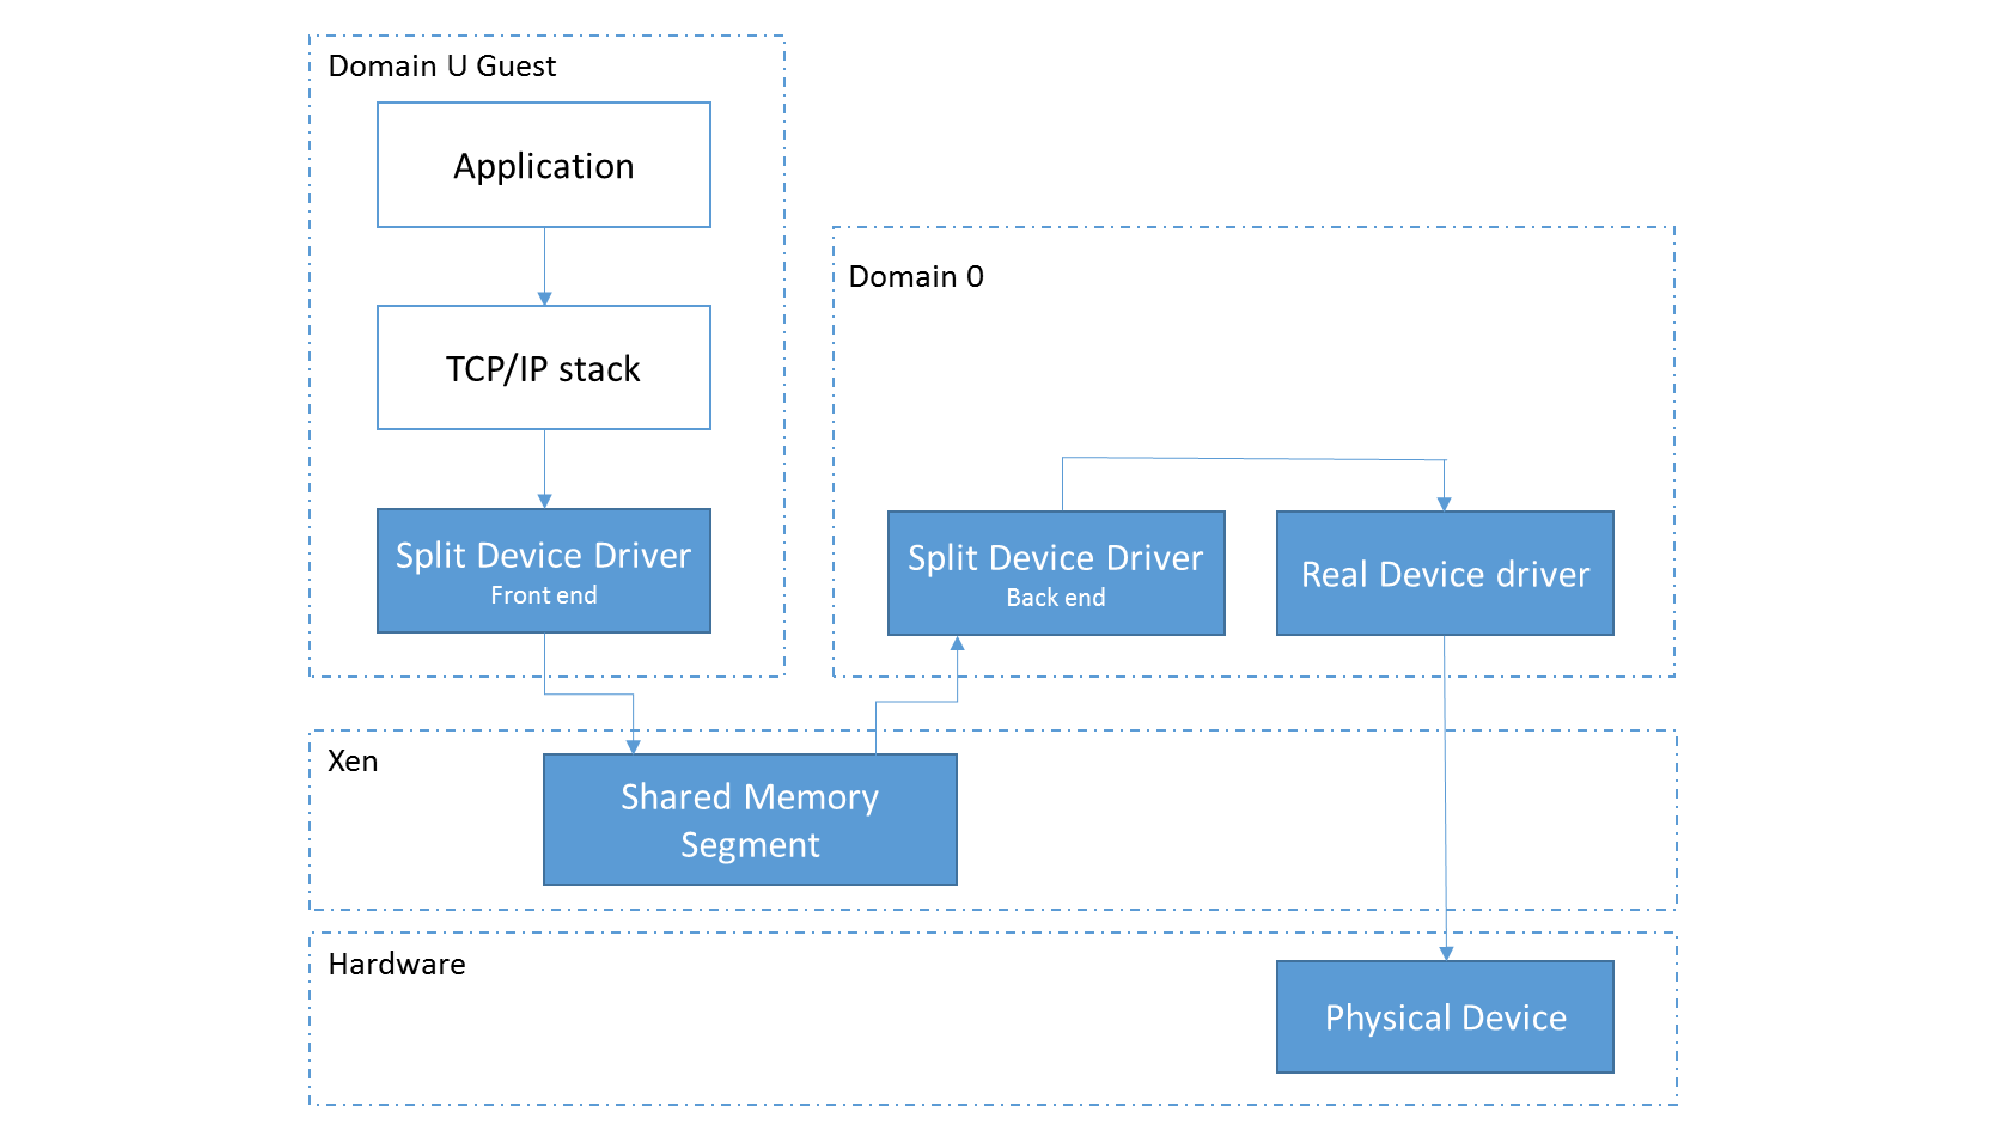
\includegraphics[scale=.50]{xen-split-tcp.pdf}
\caption{Split device driver model}
\label{fig:xen-split}
\end{figure}
Xen does not include device drivers for all the devices, adding support for all the devices would be a duplication of effort. Instead, Xen delegates hardware support to a guests. The guest typically runs in priviledged domain, although it is possible to delegate hardware to guests in other domains. Model in which hardware support is delegated to a guest is called split device driver model~\cite{Chisnall:2007:DGX:1407351}. Xen uses the same split device driver model for driver domain as shown in the figure~\ref{fig:xen-split}.
\\
Xen has a front end driver in the guest operating system and a back end driver in the driver domain. The front end and the back end driver transfer data between domains over a channel that is provided by the Xen virtual machine monitor. Within the driver domain, back end driver is used to demultiplex incoming data to the device and to multiplex outgoing data between the device and the guest domain~\cite{driverdomain}.
\\
The Xen design follows an interrupt based approach in the communication channel~\cite{Barham:2003:XAV:945445.945462}. In this communication model, front end and back end notifies each other the receipt of a service request and corresponding responses by sending an interrupt. This interrupt based model requires the context switches~\cite{Barham:2003:XAV:945445.945462}. In a multitasking system, context switch refers to the switching of the CPU from one process or thread to another. Context switch makes multitasking possible. At the same time, context switch causes unavoidable system overhead~\cite{Li:2007:QCC:1281700.1281702, Mogul:1991:ECS:106973.106982}. Hence the overhead is caused by the communication channel in the Xen driver domain. 
\\
In our proposed solution, a thread in the back end driver spins for the service request, and the front end driver spins for the availability of the corresponding responses. As a spinning does not involve any context switch, our solution performs better than the Xen device driver domain. 
\\
In this thesis, we re-implement the Xen driver domain and call it as Isolated Device Driver (IDDR). The proposed solution is implemented with IDDR as a base code.
\pagebreak

\section{Core Contributions}

The core contributions of this project are listed below. 

\begin{enumerate}
\item Re-implementation of the Xen driver domain - Isolated Device Driver (IDDR).
\item Improve the performance of IDDR by implementing thread based communication channel instead of interrupt based communication channel. 
\item The performance comparison of the thread based IDDR and interrupt based IDDR.
\end{enumerate}

\pagebreak
\section {Organization}

This section gives the organization and roadmap of the thesis.

\begin{enumerate}
\item Chapter 2 gives the background on Processes, threads, Memory protection, Virtualization, Hypervisor and inter-domain communication.
\item Chapter 3 gives the introduction to design of the system to isolate device driver. 
\item Chapter 4 discusses the detailed design and implementation to isolate device driver. 
\item Chapter 5 evaluates the performance of Independent device driver with different designs.
\item Chapter 6 reviews the related work in the area of kernel fault tolerance.
\item Chapter 7 concludes the report and lists down the topics where this work can be extended.
\end{enumerate}

\ifbool{toShowBibliography}{\bibliography{references}}{}